\section{Introducción}
\label{sec:intro}

En la presente sección se explicará cual es el contexto actual del desarrollo 
de software empresarial. Se analizará también como se organiza un sistema de 
este tipo y la técnica de reutilización de código mediante el uso de 
\dependencies.\\


\subsection{Desarrollo de sistemas web en la \jvm}
\label{subsec:intro:jvm_dev}

El presente trabajo se encuadra dentro del desarrollo de una herramienta para 
sistemas web desarrollados sobre la \jvm. La elección no es casual y responde 
a la creciente popularidad de los lenguajes que corren sobre esta plataforma. 
También influye en la decisión los cambios por los que ha transitado el
desarrollo de soluciones empresariales a lo largo de los años.\\
La plataforma de \emph{Oracle}, la \emph{Java Virtual Machine} (\jvm), permite 
correr  en ella cualquier lenguaje que compile a \bytecode \java. En 
particular, el lenguaje \java fue el primero en compilar a esta plataforma. Con 
el tiempo, muchos otros lenguajes capaces de correr en esta plataforma han 
aparecido. \scala, \clojure y \groovy  son algunos de los más populares y han 
dotado a la  plataforma de muchas nuevas herramientas y posibilidades.\\
El apéndice \ref{appendix:jvm} muestra como ha crecido esta plataforma y las 
posibilidades que ofrece.\\
Por otro lado, en la industria del software para desarrollo empresarial, las 
tecnologías web se han posicionado como la elección obvia. Esto se ha debido a 
su facilidad de desarrollo, su bajo costo, y la facilidad de crecimiento que 
presentan los sistemas desarrollados de esta forma. Todo esto se combina con 
la creación del \html5 para el desarrollo de aplicaciones web, que permite un 
alto grado de usabilidad, así como la aparición de plataformas que brindan 
servicios de hosting de alto rendimiento y escalabilidad a bajo costo.\\
Estos factores, junto con una breve reseña de la evolución de la industria del 
software empresarial se puede encontrar en el apéndice \ref{appendix:history}.

\subsection{Estructura común de sistemas web}
\label{subsec:intro:jvm_dev:structure}

La mayoría de los sistemas web suelen dividirse en capas (También llamadas
\emph{layers} o \emph{tiers}). Estas capas se dividen de forma tal que
cada una esté encargada de partes muy puntuales de la lógica de la aplicación.\\
La mayoría de los autores  suelen identificar tres capas, las cuales, 
dependiendo del autor, suelen recibir distintos nombres, aunque la estructura 
es siempre la misma. Estas capas son: la de interfaz o \view, la de \logic,
modelo o aplicación y la de \data o persistencia.\\
La capa de datos es la encargada de manejar los accesos a la base de datos, 
persistir la información, y todo lo relacionado a elementos de los que se deba 
guardar registro. La capa de lógica de negocios es la que contiene el código de 
las competencias de la aplicación, es decir, las cosas que la aplicación puede 
hacer, su funcionalidad. Finalmente, la capa de interfaz es la que permite 
acceder a la funcionalidad y visualizar los datos a los usuarios o clientes 
\citesq[pag 29-30]{Barish:2002:BOOK}. La \figref{fig:intro:jvm:web_arch} 
muestra la arquitectura básica de una aplicación web según este esquema.\\

\begin{figure}[tb]
	\centering
	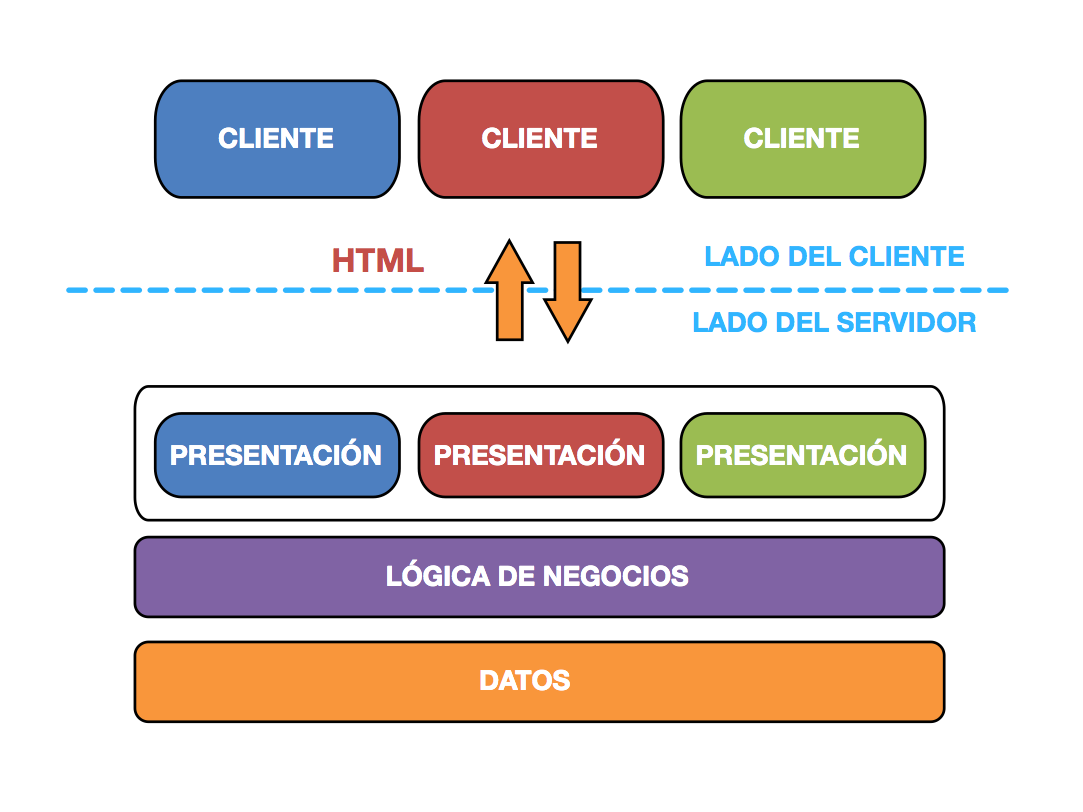
\includegraphics[]{figures/web_arch.png}
	\caption{Arquitectura em capas básica de un sistema web.}
	\label{fig:intro:jvm:web_arch}
\end{figure}
 
El presente trabajo se enfocará en la \viewtier, aunque utilizará conceptos 
desarrollados para la \logictier para su desarrollo.
 
\subsection{Reutilización de código mediante \dependencies}
\label{subsec:intro:jvm_dev:dependencies}

Existen numerosos \frameworks, \toolkits, bibliotecas y porciones de código 
que los desarrolladores pueden utilizar en el código de su proyecto, de forma 
de obtener funcionalidades genéricas previamente desarrolladas. Estas porciones 
de código de terceros que utilizan los desarrolladores en sus proyectos reciben 
el nombre de \dependencies.\\
En este trabajo se identificaran dos tipos de dependencias. las de la 
\logictier, dadas por \emph{paquetes} de código \java compilado (archivos .jar 
o .war), y las de \viewtier que consisten en (pero no se limitan a) archivos 
\css y \js. A su vez, estas dependencias pueden ser manejadas o no manejadas.\\
Las \dependencies no manejadas son código que se agrega manualmente al
proyecto mediante la clásica técnica de \quoted{copiar y pegar} o agregando los 
archivos correspondientes a esa \dependency en alguna carpeta del proyecto 
(Proceso al que se denominará \quoted{instalar}). Por su parte, las 
\dependencies manejadas consisten en algún tipo de descripción en un \conffile 
o símil que declarará el código de terceros requerido. Un programa externo 
evaluara el \conffile al momento de la compilación y se encargará de descargar 
e \emph{instalar} las \dependencies declaradas. Estos programas son
conocidos como \depmgrs.\\
La figura siguiente muestra de forma gráfica los tipos de \dependencies para 
una mejor comprensión de lo previamente expresado.
\jump[2]

\begin{forest}
	for tree={
		draw,
		minimum height=2cm,
		anchor=north,
		align=center,
		child anchor=north
	},
	[{\dependencies}, align=center, name=Deps
		[{\dependencies de la\\\logictier}, name=LogDeps
			[{\dependencies\\no manejadas}, name=LogDepsManaged]
			[{\dependencies\\manejadas}, name=LogDepsNotManaged]
		]
		[{\dependencies de la\\\viewtier}, name=ViewDeps
			[{\dependencies\\no manejadas}, name=ViewDepsManaged]
			[{\dependencies\\manejadas}, fill=yellow, name=ViewDepsNotManaged]
		]
	]
\end{forest}

\jump[2]
Las \dependencies no manejadas implican una serie de pasos repetitivos y 
propensos a errores que el usuario debe realizar con el objetivo de poder 
correr su código. Por su parte, las \dependencies manejadas son preferentes, ya 
que eliminan errores comunes y ahorran tiempo y trabajo a los desarrolladores. 
Además, los \depmgrs suelen simplifican la complejidad asociada a instalar las 
\dependencies anidadas\footnote{
	Asuma el lector un proyecto \emph{A} con una \dependency \emph{B}. El 
	paquete \emph{B} es a su vez un proyecto con \dependencies, por ejemplo 
	\emph{C}. Para que \emph{A} funcione correctamente, requiere \emph{B} y 
	este a su vez requiere \emph{C}, haciendo que de forma transitiva \emph{A} 
	requiera \emph{C}.
} \citesq{Larman:2010:BOOK}.\\
Las \dependencies de la \viewtier en la plataforma \java, suelen ser no 
manejadas. El presente trabajo se enfoca en transformar esas dependencias, en 
dependencias manejadas.\\
El anexo \ref{appendix:depmgmnt} muestra como funcionan los distintos \depmgrs
en las diferentes capas de aplicación.
